\subsection{Dublin City Parking Information}
There are various parking data required for the simulation. The list below outlines the data and the reason why they are required. The succeeding section explains the process in obtaining the data.

\begin{itemize}
    \item Parking Area Geographic Coordinates: In order to simulate vehicles parking in areas that allow parking, all Dublin on-street parking locations as well as parking lot locations must be known. The coordinate locations are recorded so that vehicles may be able to calculate which parking areas are closest to their final destination during the simulation.
    \item Parking Area Capacities: The parking space capacity of each parking lot and on-street location is recorded. The capacities are used to determine how full a parking area is throughout the simulation process.
    \item Parking Area SUMO Road ID: The SUMO road identifiers must be recorded for each parking area so that the vehicles may be routed to them. SUMO road identifiers is the only accepted parameter for the function for routing vehicles dynamically within the simulation.
\end{itemize}

\subsubsection{On-Street Parking Information}\label{ssec:on-street_parking_info}
data.gov.ie offers various datasets for transport data in Ireland. The most granular transport dataset regarding on-street parking locations is the parking meters dataset \{CITE\}. It does not contain the precise locations of each individual parking spot, but it has the locations of every parking meter within Dublin city. More specifically, the dataset includes Irish grid reference coordinates of all parking meters as well as the number of on-street parking spaces that they serve. Thus this dataset is sufficient for the purpose of this simulation. The dataset is also substantial as it references all known parking meters in Dublin. The area of interest for this dissertation is inner city Dublin parking areas. This can be visualised as the ``yellow" and ``red" areas in terms of \ac{dcc} defined parking zones as shown in figure \ref{fig:DUBLINZONES}. 

The resultant dataset within the concerned zones includes 175 on-street parking meters that serve 12,289 parking spaces. Each parking meter coordinate is formatted to an Irish coordinate reference plane. For the data to be usable in this dissertation, they must be converted to the more commonly used geographic coordinate system. Online tools are available to complete this conversion process.

The SUMO road identifiers are obtained through a manual mapping process of each parking meter through the SUMO GUI.

\begin{figure}[H]
    \centering
    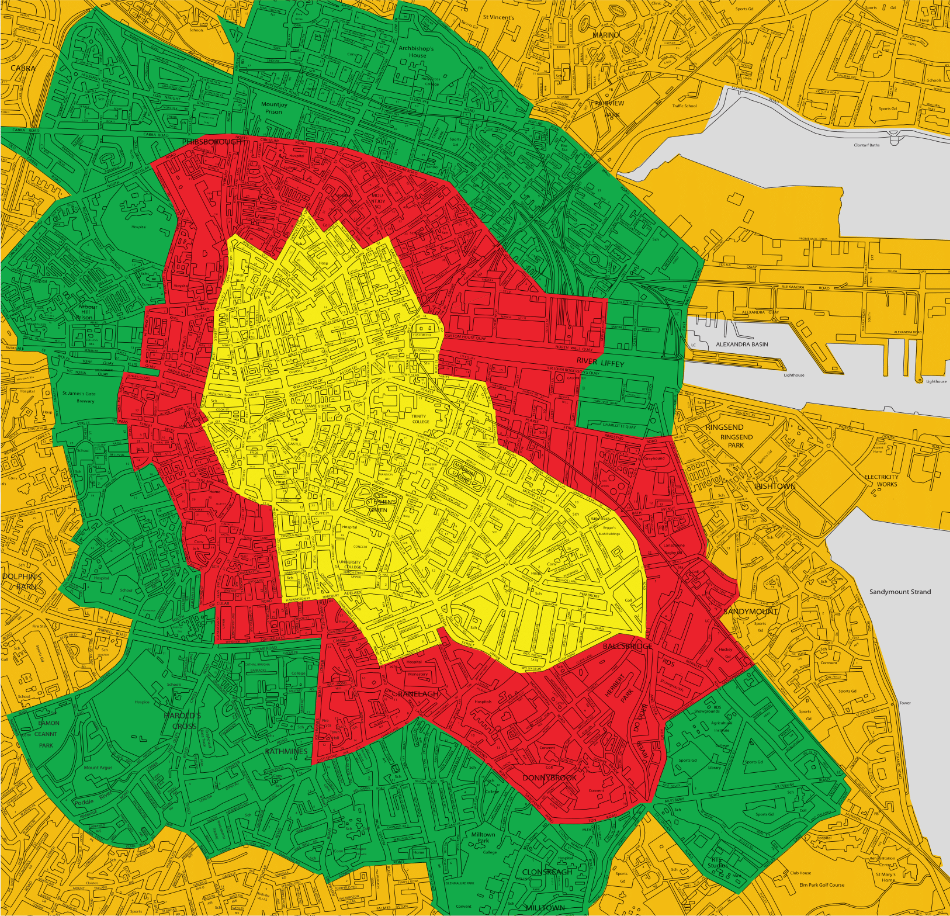
\includegraphics[width=\textwidth]{./Images/DUBLINZONES.PNG}
    \caption{Dublin City Council Parking Zones Breakdown \citep{DublinTariffs}}
    \label{fig:DUBLINZONES}
\end{figure}

\subsubsection{Car Park Information}\label{ssec:car_par_cap}
There are 14 parking lots that this dissertation takes into account. Table \ref{table:carpark} includes the 14 parking lots and their capacities.

\begin{table}[H]
    \begin{center}
        \begin{tabular}{||c c||} 
            \hline
            Car Park & Capacity\\ [0.5ex] 
            \hline\hline
            Arnotts Department Store & 500\\ 
            \hline
            Christ Church &  212\\
            \hline
            ILAC Shopping Centre & 1000 \\
            \hline
            Parnell Street & 500 \\
            \hline
            Marlboro Street & 567 \\
            \hline
            Abbey Street & 340 \\
            \hline
            Thomas Street & 230 \\
            \hline
            Setanta & 145 \\
            \hline
            Trinity Street & 252 \\
            \hline
            Stephen's Green & 1127 \\
            \hline
            Brown Thomas & 380 \\
            \hline
            Dawson Street & 370 \\
            \hline
            Jervis Shopping Centre & 264\\ [1ex]
            \hline
        \end{tabular}
        \caption{Dublin Parking Lots and Capacities}
        \label{table:carpark}
    \end{center}
\end{table}

Most of the car parks in Dublin are operated by QPark. Information regarding their capacities are available on each of the corresponding QPark parking lot websites. Other car parks are operated by the shopping centres that they they serve and the capacities of them are listed on the corresponding shopping centre websites.

The coordinates of each of the car park locations are recorded through Google Maps.

The SUMO road identifiers are obtained through a manual mapping process of each car park through the SUMO GUI.
